\newpage
\section{Resultados}

\subsection{4-PAM com codificação binária}

Na figura \ref{fig:sinais1}, são mostrados os sinais do sistema PAM com codificação binária. Como pode-se notar na legenda observa-se os pontos onde ocorreu a leitura de sinal. Como nota-se quando comprara-se o sinal transmitido ao recebido, percebe-se um atraso de aproximadamente 6 bits.

\begin{figure}[H]
    \centering
    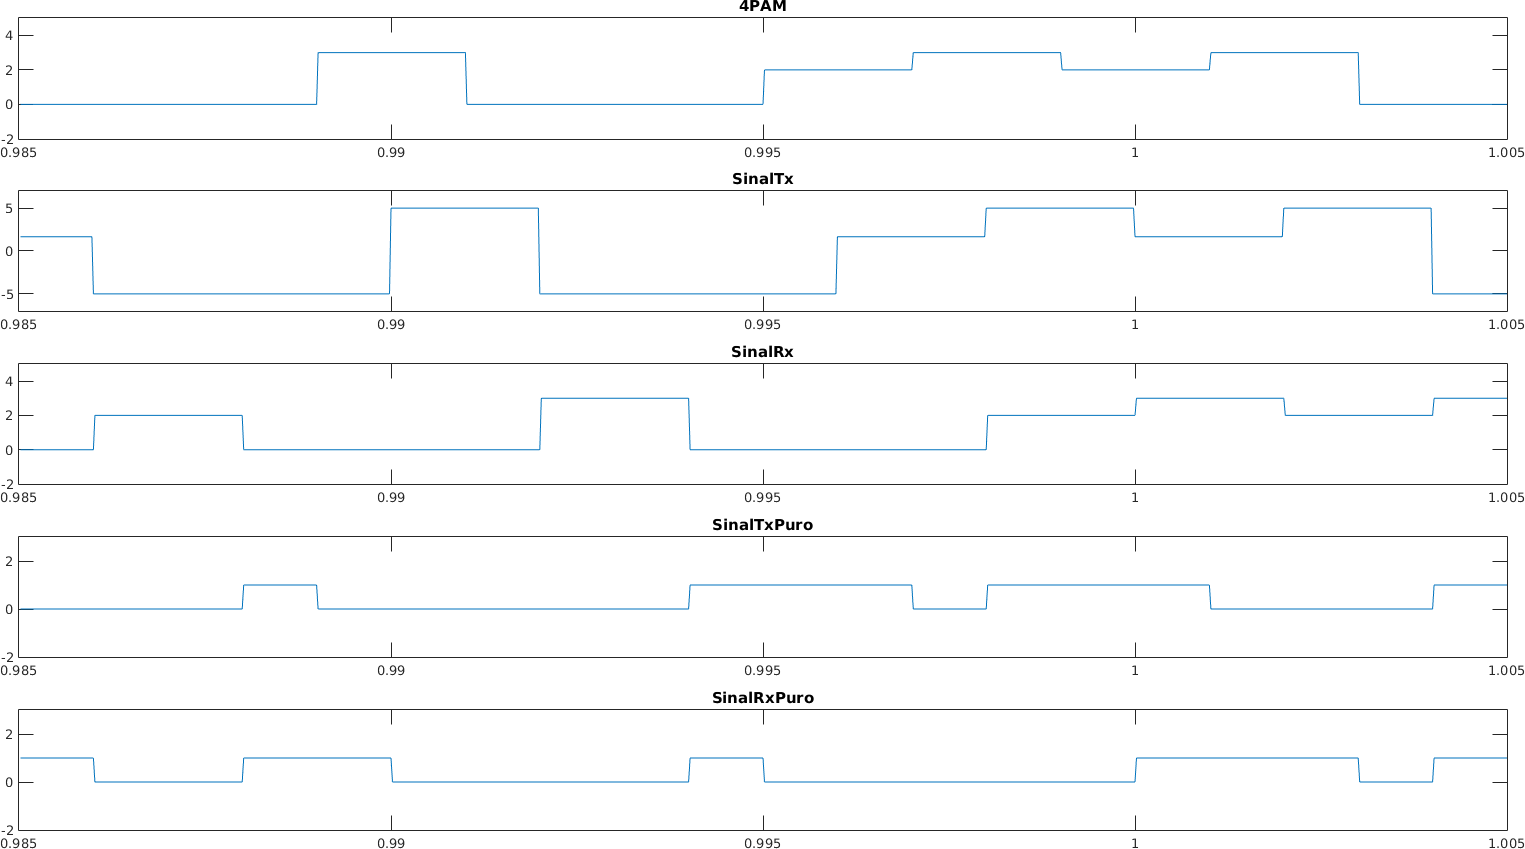
\includegraphics[scale=0.4]{sinalbin}
    \caption{Sinais obtidos.}
    \label{fig:sinais1}
\end{figure}

Quanto ao desempenho do sistema, a tabela \ref{tab:3} mostra a taxa de erro de bit e a probabilidade de erro em função da razão energia de bit e potência do ruído, sendo que a figura \ref{fig:bin} mostra a representação gráfica da BERx$\frac{Eb}{No}$.

\begin{small}
    \begin{table}[H]
        \begin{center}
            \caption{Tabela BER x Eb/No}
            \begin{tabular}{c|c|c}
                \hline
                $\frac{Eb}{No}$ [dB] & BER & $P_b$ \\
                \hline
                $\infty$ & 0 & 0 \\
                \hline
                10 & 0.0031  & $2.4 \times 10^{-3} $ \\
                \hline
                8 & $1.28 \times 10^{-3}$ & 0.0123 \\
                \hline
                6 & 0.0396 &  0.0372 \\
                \hline
                4 & 0.077 &  0.0782 \\
                \hline
                2 & 0.1311 & 0.1301 \\
                \hline
                0 & 0.1821 & 0.1855 \\
                \hline
            \end{tabular}
            \label{tab:3}
        \end{center}
    \end{table}
\end{small}

\begin{figure}[H]
    \centering
    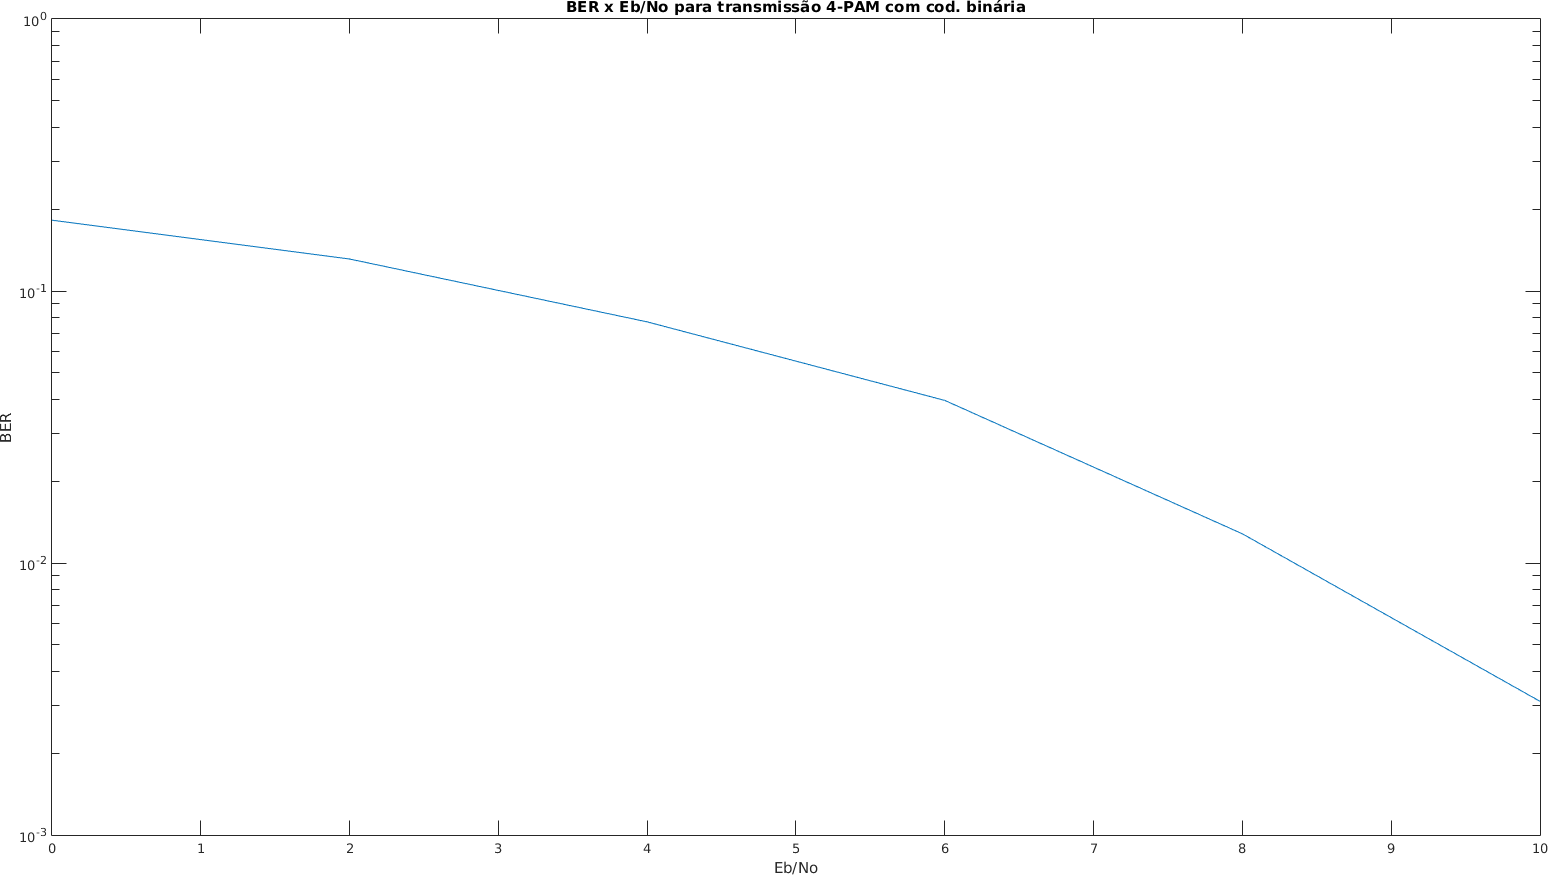
\includegraphics[scale=0.4]{bin}
    \caption{BER com código binário.}
    \label{fig:bin}
\end{figure}



\subsection{4-PAM com codificação Gray}

Na figura \ref{fig:sinais2}, são mostrados os sinais do sistema PAM com codificação gray. Como pode-se notar na legenda observa-se os pontos onde ocorreu a leitura de sinal. Como nota-se quando comprara-se o sinal transmitido ao recebido, percebe-se um atraso de aproximadamente 6 bits.

\begin{figure}[H]
    \centering
    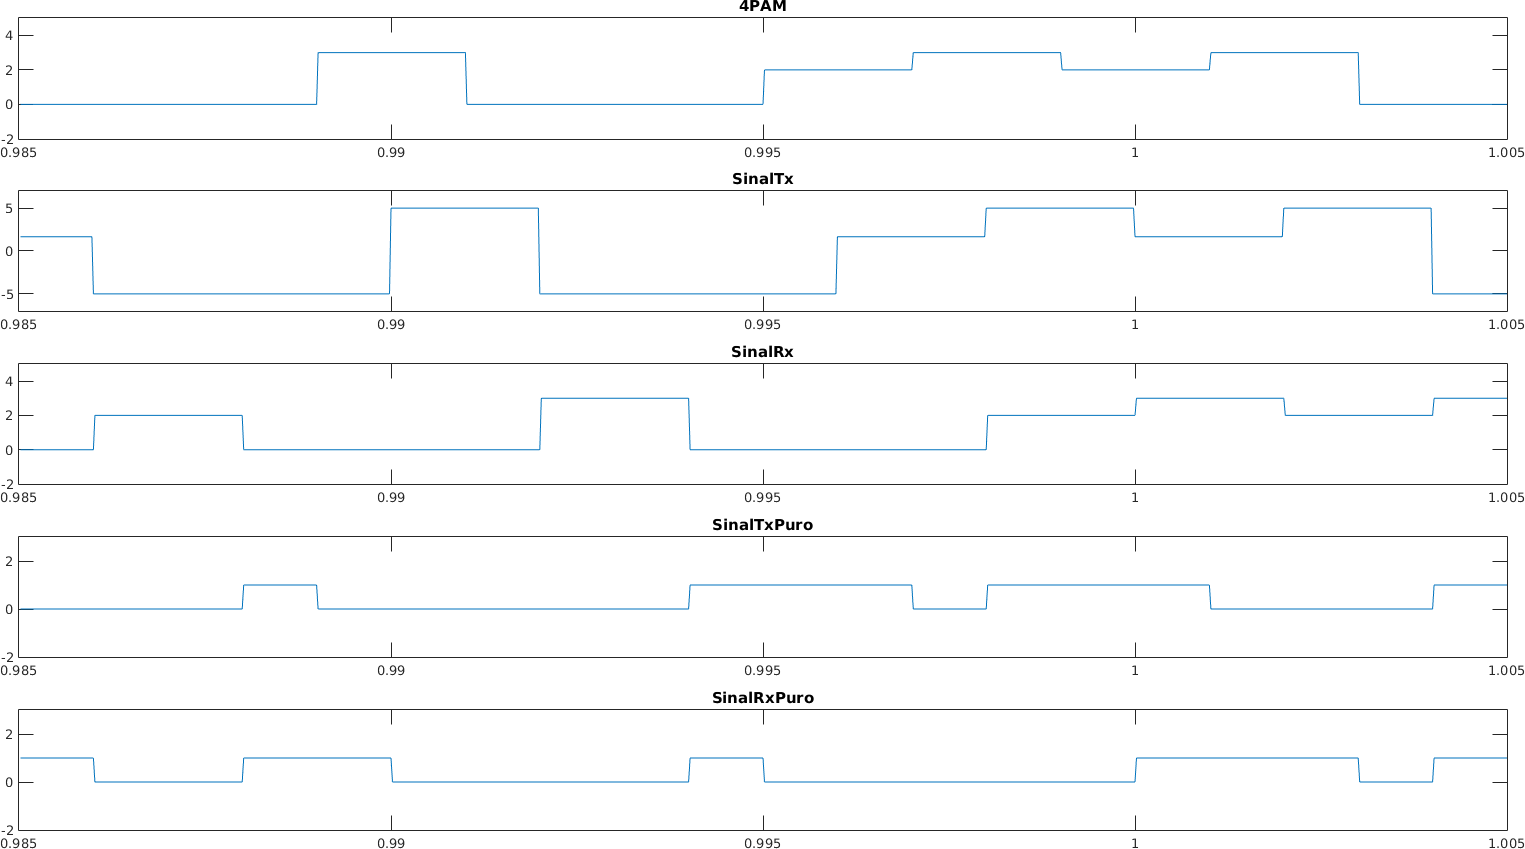
\includegraphics[scale=0.4]{sinalgray}
    \caption{Sinais obtidos.}
    \label{fig:sinais2}
\end{figure}

Quanto ao desempenho do sistema, a tabela \ref{tab:4} mostra a taxa de erro de bit e a probabilidade de erro em função da razão energia de bit e potência do ruído, sendo que a figura \ref{fig:gray} mostra a representação gráfica da BERx$\frac{Eb}{No}$.

\begin{small}
    \begin{table}[H]
        \begin{center}
            \caption{Tabela BER x Eb/No}
            \begin{tabular}{c|c|c}
                \hline
                $\frac{Eb}{No}$ [dB] & BER & $P_b$ \\
                \hline
                $\infty$ & 0 & 0 \\
                \hline
                10 & 0.0019 & $1.8 \times 10^{-3} $ \\
                \hline
                8 & $8.6 \times 10^{-3}$ & 0.0092 \\
                \hline
                6 & 0.0274 &  0.0279 \\
                \hline
                4 & 0.0595 & 0.0586 \\
                \hline
                2 & 0.0954 & 0.0976 \\
                \hline
                0 & 0.1463 & 0.1392 \\
                \hline
            \end{tabular}
            \label{tab:4}
        \end{center}
    \end{table}
\end{small}

\begin{figure}[H]
    \centering
    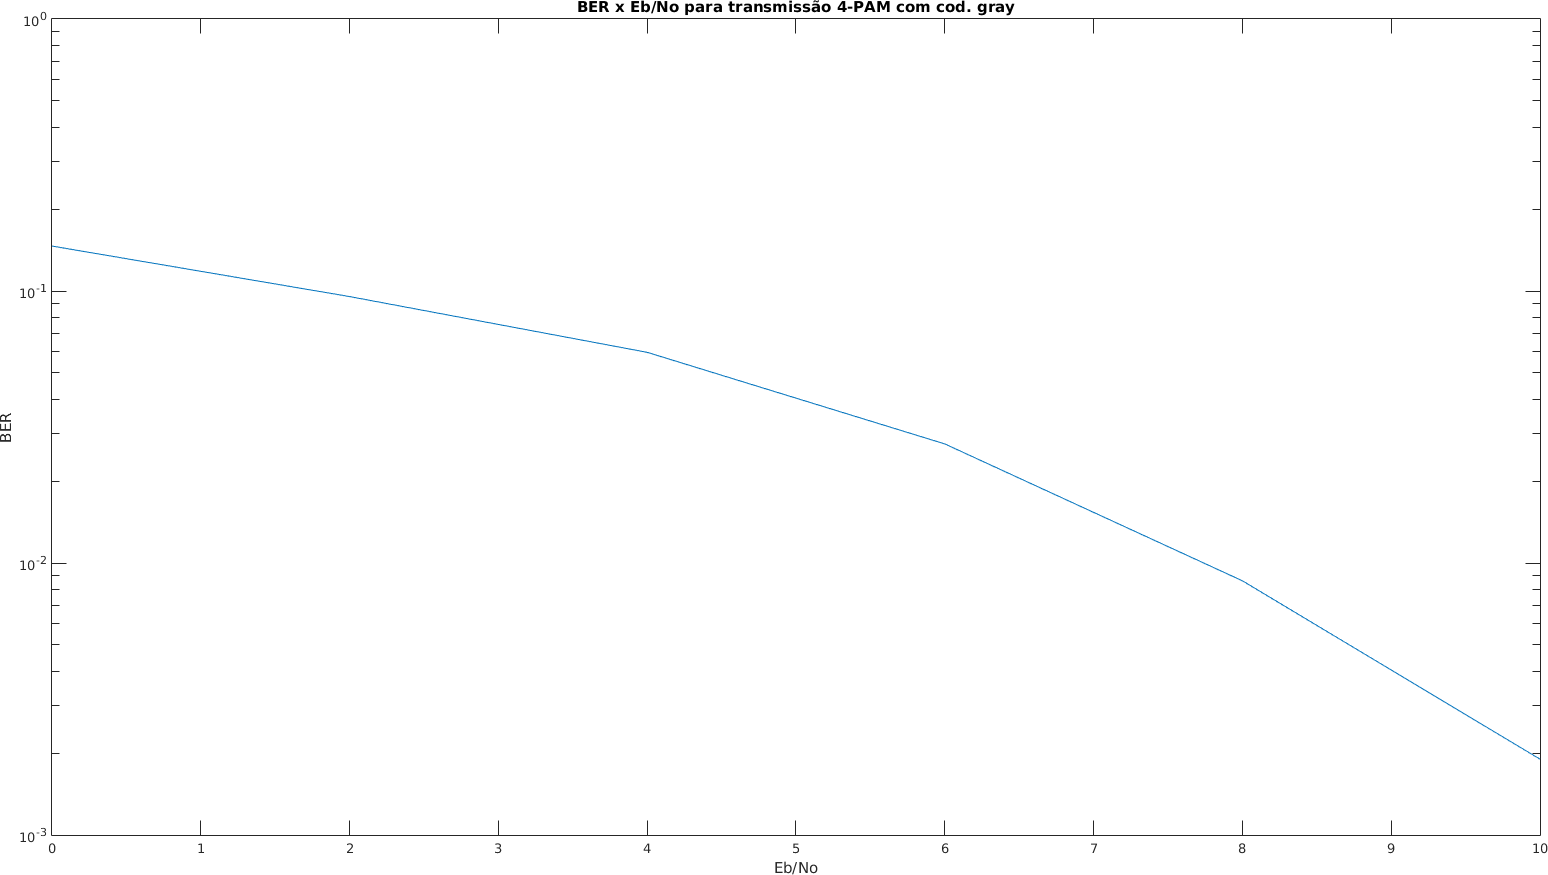
\includegraphics[scale=0.4]{gray}
    \caption{BER com código Gray.}
    \label{fig:gray}
\end{figure}


Para finalizar, a figura \ref{fig:bxg} mostra o gráfico de desempenho para as duas codificações, onde nota-se claramente a vantagem da codificação gray em relação a codificação binária.

\begin{figure}[H]
    \centering
    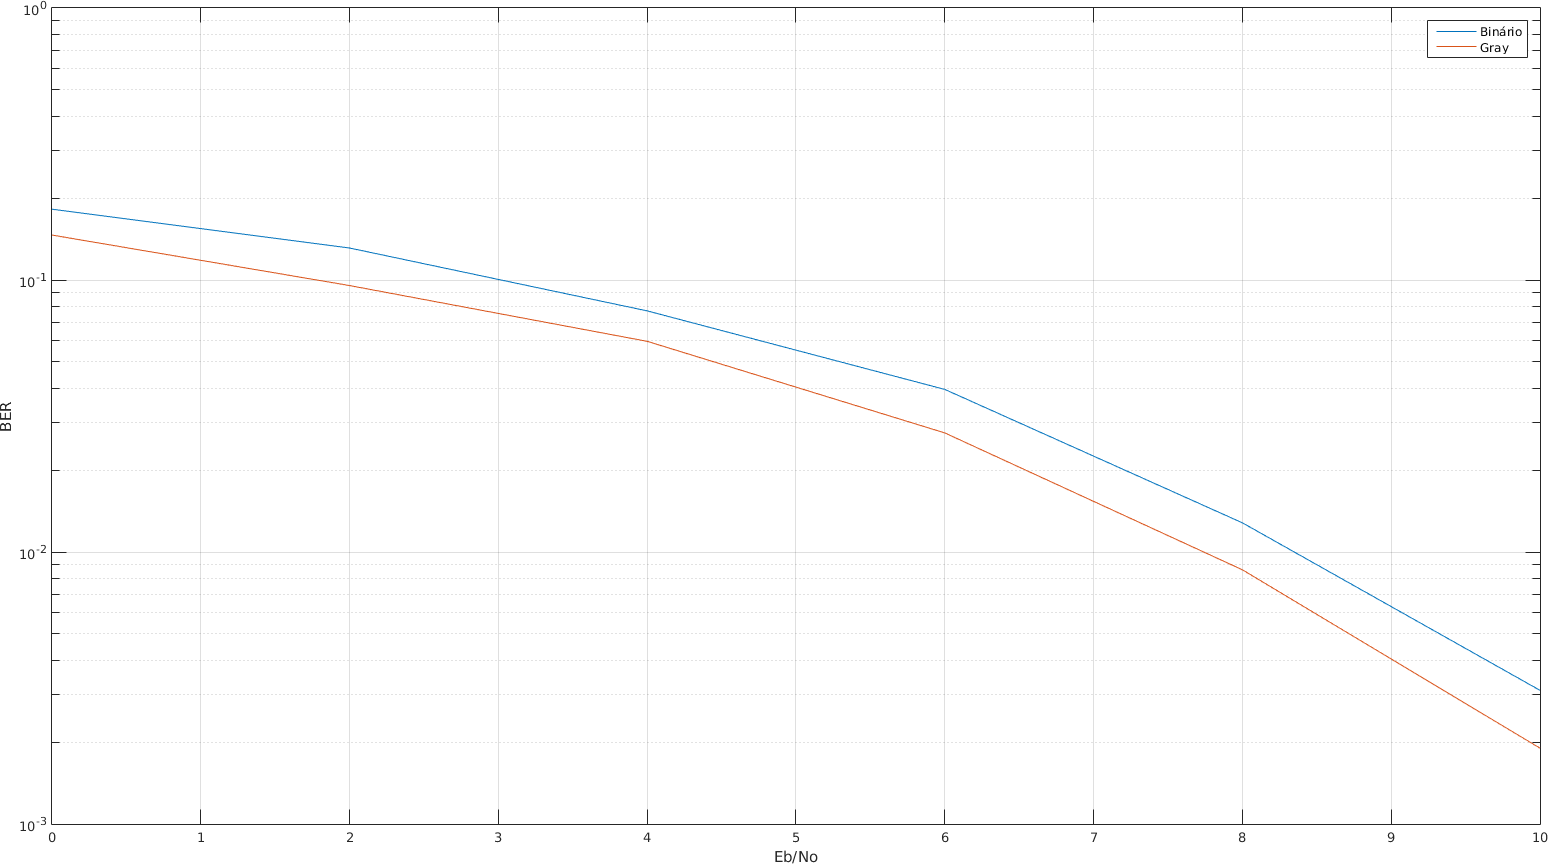
\includegraphics[scale=0.4]{bxg}
    \caption{Exemplo de figura}
    \label{fig:bxg}
\end{figure}